\section{Hardware urządzenia}
\label{sec:hardware}
Urządzenia zostały wykonane samodzielnie. Powstały dwa prototypy, pierwszy znacznie większy oferuje podobną funkcjonalność do drugiego. 

\subsection{Pierwszy prototyp}

Schemat płytki PCB tego prototypu przedstawia \autoref{fig:pcb_1}. Płytka ta jest trzykrotnie większa od prototypu w wersji drugiej \autoref{fig:pcb_2}. Widać, że odległości między ścieżkami zostały skompresowane do minimum. 

\begin{figure}[!htbp]
	\centering
	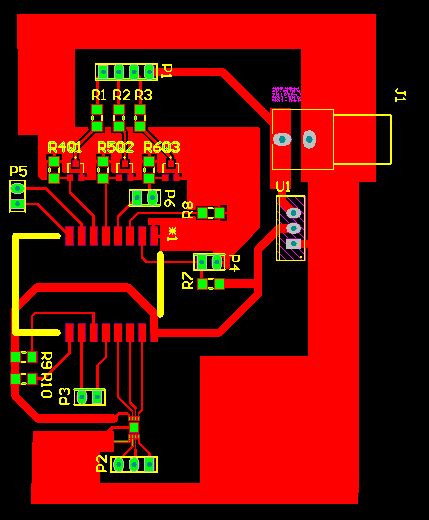
\includegraphics[width=0.5\textwidth]{images/fig02-PCBv1.png}
	\caption[Schemat płytki PCB v1.]{Schemat płytki PCB w wersji I}
	\label{fig:pcb_1}
\end{figure}


\subsection{Drugi prototyp}

\begin{figure}[!htbp]
	\centering
	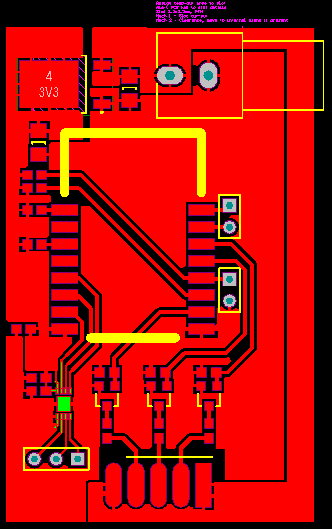
\includegraphics[width=0.3\textwidth]{images/fig03-PCBv2.png}
	\caption[Schemat płytki PCB v2.]{Schemat płytki PCB w wersji II}
	\label{fig:pcb_2}
\end{figure}

\subsection{Schemat układu}


\begin{figure}[!htbp]
	\centering
	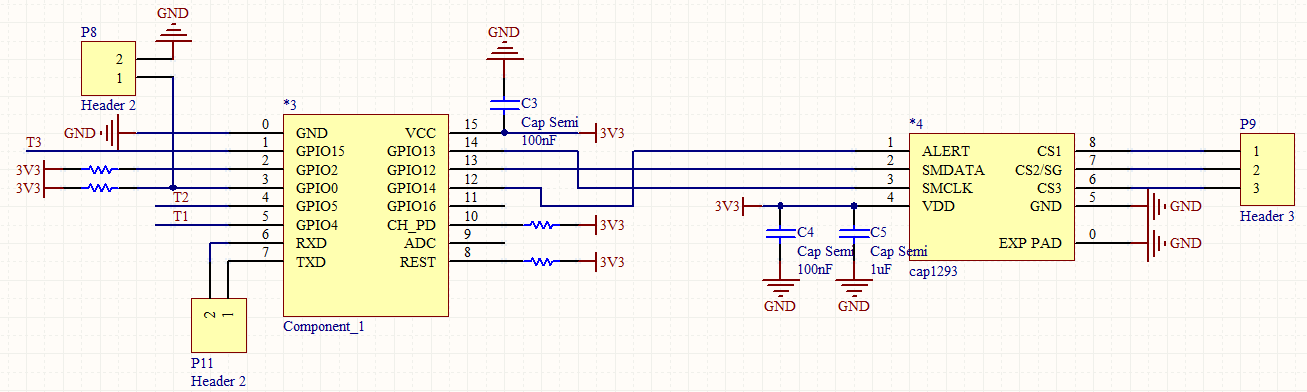
\includegraphics[width=1.0\textwidth]{images/fig04-schemat.png}
	\caption[Schemat układu urządzenia.]{Schemat układu urządzenia}
	\label{fig:schemat_pcb}
\end{figure}

Schemat układu urządzenia przedstawia \autoref{fig:schemat_pcb}. Mamy tutaj przedstawione urządzenie \texttt{ESP8266} (Component 1), piny \texttt{Reset}, \texttt{CHPD} oraz \texttt{VCC} podpięte są do napięcia wysokiego 3,3V. Piny oznaczone jako \texttt{T1}, \texttt{T2}, \texttt{T3} to wyprowadzenia do tranzystorów, które sterują kolorami diod LED RGB. Piny \texttt{{RXD} oraz \texttt{TXD} służą do wgrywania programu, wykonuje się to komendą 
\begin{lstlisting}
sudo ./luatool.py -p /dev/ttyUSB0 -f init.lua -t init.lua
\end{lstlisting} 
Narzędzie luatool\cite{luatool-www} służy do wgrywania pliku init.lua do środowiska nodemcu\cite{nodemcu-www} 
Aby mieć możliwość wgrania środowiska nodemcu\cite{nodemcu-www} do układu ESP8266 należy zewrzeć zworkę (Header 2)
